\documentclass[12pt]{article}		%this tells latex what kind of document to create
\usepackage{amsmath} %even more math
\usepackage{amsthm} %for theorems
\usepackage{array}
\usepackage{authblk}
\usepackage[english]{babel}
\usepackage{calc}
\usepackage{caption}
\usepackage[usenames,dvipsnames]{color} % Required for custom colors
\usepackage{dcolumn}
\usepackage{enumitem,linegoal} % Used for alphabetical lists instead of numbered lists in {itemize}
\usepackage{extramarks} % Required for headers and footers
\usepackage{fancyhdr} % Required for custom headers
\usepackage{float}
\usepackage{framed}
\usepackage[margin=1in]{geometry} %1 inch margins
\usepackage{graphicx} % Required to insert images \includegraphic
\usepackage[hidelinks]{hyperref}
\usepackage[utf8]{inputenc}
\usepackage{lastpage} % Required to determine the last page for the footer
\usepackage{listings} % Required for insertion of code
\usepackage{longtable}
\usepackage{mathtools} %math things
\usepackage{multirow,bigdelim}% allows tables to have a column spanning multiple rows
\usepackage[round]{natbib} %for soc sci bibliography
\usepackage{outlines}
\usepackage{pgfgantt}
\usepackage{pdflscape}
\usepackage{pgfplots} % packages for graphing
\usepackage[section]{placeins}
\usepackage{rotating} %lets you rotate floats (tables, figures) pages
\usepackage{sectsty}
\usepackage{setspace}
\usepackage{siunitx} %units! 
\usepackage{subcaption} %allows for subtables and subfigures
\usepackage{tikz} % packages for graphing
\usepackage{titlesec}
\usepackage{todonotes} %gives missing figure

\allsectionsfont{\singlespacing}
\DeclareMathOperator{\Lagr}{\mathcal{L}}
\DeclareMathOperator{\sumn}{\sum_{i=1}^n}
\DeclareMathOperator{\bh}{\hat{\beta}}
\DeclareMathOperator{\yh}{\hat{y}}
\DeclareMathOperator{\ybar}{\bar{y}}
\DeclareMathOperator{\xbar}{\bar{x}}
\graphicspath{ {figures/} }
\linespread{2}
\newcommand{\mathnode}[1]{%
	\mathord{\tikz[baseline=(#1.base), inner sep = 0pt]{\node (#1) {$#1$};}}}
\setcounter{secnumdepth}{4}
\tikzset{every picture/.style=remember picture}
\renewcommand{\theenumi}{\Roman{enumi}. }
\renewcommand{\labelenumi}{\theenumi}
\renewcommand{\theenumii}{\Alph{enumii}. }
\renewcommand{\labelenumii}{\theenumii}
\renewcommand{\theenumiii}{\roman{enumiii}. }
\renewcommand{\labelenumiii}{\theenumiii}
\renewcommand{\theenumiv}{\alph{enumiv}) }
\renewcommand{\labelenumiv}{\theenumiv}
\usetikzlibrary{arrows} % packages for graphing
\usetikzlibrary{calc} % packages for graphing
\usetikzlibrary{decorations.pathreplacing} % packages for graphing
\usetikzlibrary{shapes.geometric}
\usetikzlibrary{shapes.misc} 	%Reads the document `preamble.tex' into this document. This is where I load packages

\title{ECO 530 - Introduction to Econometrics \\ Fall 2023 \\Exercise 4}
\author{50 points}
\date{Due Date: Friday, October 27 }


\begin{document}		%Start document
\maketitle

\section*{Instructions}
Complete the exercises below using the Nicaragua Rural Business Development Data (NicaRBD.RData). Be sure to show all of your work. For this assignment, you should submit:
\begin{itemize}
	\item A PDF containing your written answers, tables, and figures along with the R script that generates them.
\end{itemize}


\clearpage

\section*{Example}

Consider the following equation depicting the relationship between an outcome $y_i$ and an explanatory variable $x_i$

$$ y_i = \beta_0 + \beta_1 x_i + \epsilon_i$$

Imagine that you obtain estimates of $\beta_0$ and $\beta_1$ via OLS. You can use those estimates ($\bh_0,\bh_1$) to predict $y$ for any level of $x$. Remember, this is our guess at the value of $E[y|x]$

$$ \yh_i = \bh_0 + \bh_1 x_i $$

We can sketch our estimated relationship as:

\begin{center}
	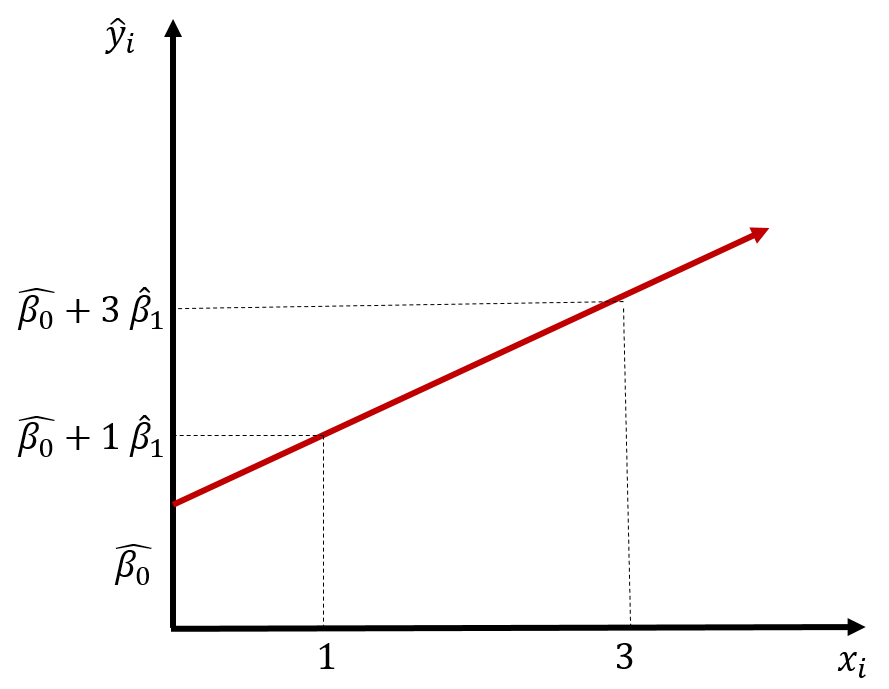
\includegraphics[width=.5\textwidth]{example.png}
\end{center}

That is, a line with its intercept at $\bh_0$ and a slope of $\bh_1$. 

\clearpage


\section*{Q1 - Prepare the data}

In these exercises, we are going to be working with the variables listed below. Food expenditure will serve as the outcome variable in all of your regressions. Create a data frame without missing values on these variables. Present a table of summary statistics and briefly describe the data in a paragraph.

\begin{itemize}
	\item food.expend - Expenditure on food measured in purchasing power parity (PPP) adjusted dollars
	\item land - A respondent's landholding, measured in \textit{manzanas}.
	\item hadloan - Equal to one if a respondent had a loan and zero otherwise
	\item crop - A factor variable with values 1-4 and labels ``Beans'', ``Livestock'', ``Sesame'', and ``Casava''
\end{itemize}


\clearpage

\section*{Q2 - A single continuous regressor}

Estimate the relationship between food expenditure and land holding via Ordinary Least Squares. Explicitly discuss your decision regarding whether or not to use heteroskedasticity robust standard errors. Report and discuss your results. Then, as in the example, plot or sketch the relationship you estimated.

\clearpage

\section*{Q3 - Add a binary control variable}

Estimate the relationship between food expenditure and land holding again, this time conditioning on whether the respondent had a loan. Report and discuss your results. How do they differ from your estimates in Q2? Plot or sketch the relationship you estimated again. (Hint: You'll need to draw two lines this time.).

\clearpage

\section{Q4 - Add a categorical control variable with more levels}

Estimate the relationship between food expenditure and land holding again, this time conditioning on the crop a respondent produced. Report and discuss your results. Plot or sketch the relationship you estimated again.	

\clearpage

\section*{Q5 - Interaction terms}

Estimate the specification below:

$$food.expend_i = \beta_0 + \beta_1 land_i + \beta_2 hadloan_i + \beta_3 land_i \times hadloan_i + \epsilon_i$$
 
There are various ways to create the interaction term that you'll need to estimate $\beta_3$. You could:
\begin{itemize}
	\item[1.] Create it by hand: use \textit{mutate()} to define a new variable equal to $land_i \times hadloan_i$
	\item[2.] Write the equation in your \textit{lm\_robust()} function as \textit{food.expend~land*hadloan}. R will estimate the saturated model for you.
\end{itemize}

I prefer Option 1, as I feel it gives me better control. Report and discuss your results. Plot or sketch the relationship you estimated. Explicitly test the hypothesis that the effect of landholding of food expenditure is the same for respondents with and without a loan. Finally, make a coefficient plot showing the estimated effect of landholding on food expenditure for respondents with and without a loan. 

	

\end{document}	%End document